\documentclass[10pt, letterpaper]{article}
\usepackage[margin=1in, top=0.9in, bottom=0.9in]{geometry}
\usepackage{amsmath, amssymb}
\usepackage{booktabs}
\usepackage{graphicx}
\usepackage{float}
\graphicspath{{../outputs/figures/}}
\usepackage{hyperref}
\usepackage{enumitem}
\usepackage{titlesec}
\usepackage{parskip}
\usepackage{microtype}
\usepackage{array}
\usepackage[numbers, sort&compress]{natbib}

\setlength{\parskip}{4pt}
\setlength{\parindent}{0pt}
\titlespacing*{\section}{0pt}{10pt}{4pt}
\titlespacing*{\subsection}{0pt}{7pt}{2pt}
\titleformat{\section}{\normalsize\bfseries}{\thesection.}{0.5em}{}
\titleformat{\subsection}{\normalsize\itshape}{\thesubsection}{0.5em}{}

\hypersetup{colorlinks=true, linkcolor=blue, citecolor=blue, urlcolor=blue}

\begin{document}

% ── Title ────────────────────────────────────────────────────────────────────
\begin{center}
{\large \textbf{Predicting WDR91 Binders from DNA-Encoded Library Screens\\
Using Fingerprint Models, Similarity Search, and Graph Neural Networks}}\\[8pt]
Dheeraj Malle Rudrappa (\texttt{dmall6@uic.edu}) \quad
Gautham Satyanarayana (\texttt{gsaty@uic.edu})
\end{center}

% ── Abstract ─────────────────────────────────────────────────────────────────
\section*{Abstract}
Identifying small-molecule binders for protein targets is a fundamental challenge in drug discovery. We address the DREAM Target 2035 Challenge, which tasks participants with predicting active binders for the WD40-repeat domain protein WDR91 using a DNA-Encoded Library (DEL) screen of 375,595 compounds. We hypothesised that combining fingerprint-based machine learning with structural similarity to confirmed WDR91 binders would outperform either approach alone. We trained XGBoost and LightGBM classifiers on multi-fingerprint feature vectors (ECFP6+MACCS+RDK, 4,263 bits) under a stratified 80/20 split, achieving an Enrichment Factor at 1\% (EF@1\%) of 7.98 with XGBoost. We further applied Tanimoto similarity scoring against 177 known WDR91 actives and pseudo-label-trained a Graph Convolutional Network (GCN) on the 339,258-compound Step~2 test library. The three approaches identified largely non-overlapping top-ranked candidates (GNN top~1\% overlaps only 9.4\% with the XGBoost--Tanimoto ensemble), supporting our hypothesis that combining complementary signals improves coverage of the binding chemical space.

% ── Introduction ──────────────────────────────────────────────────────────────
\section{Introduction}
Drug discovery traditionally requires expensive and time-consuming experimental screening of large compound collections. DNA-Encoded Library (DEL) technology accelerates early-stage hit identification by affinity-selecting millions of barcoded compounds simultaneously~\cite{Goodnow2017}. Machine learning on DEL data can extrapolate binding signals beyond screened compounds, enabling virtual screening of much larger libraries~\cite{McCloskey2020}.

WDR91 is a WD40-repeat domain protein involved in endosomal signalling~\cite{Jia2016}. Its shallow, hydrophobic binding pocket presents a challenging target for structure-based methods, motivating data-driven approaches. The DREAM Target 2035 Challenge~\cite{DREAM2035} provides a DEL screen of WDR91 as training data and asks participants to rank a 339,258-compound commercial library for experimental follow-up.

A central challenge is \emph{domain shift}: the training data consists of combinatorial DEL compounds assembled from three building blocks, whereas the test library contains drug-like commercial molecules from a chemically distinct space. Fixed-length fingerprints, while effective on in-distribution data, may miss structural motifs relevant to binding in the target domain. Graph Neural Networks (GNNs)~\cite{Gilmer2017} learn representations directly from molecular graphs and can in principle generalise across chemical domains.

We hypothesised that (1) XGBoost trained on multi-fingerprint features would achieve strong EF@1\% on DEL data, and (2) combining this with structural similarity to 177 confirmed WDR91 binders and a GNN trained via pseudo-labelling on the test library SMILES would identify a broader and more drug-like set of candidate binders than fingerprint models alone.

% ── Methods ───────────────────────────────────────────────────────────────────
\section{Methods}

\subsection{Data}
The WDR91 DEL training set comprises 375,595 compounds with binary hit labels (28,778 hits; 7.66\%; 12:1 imbalance) across 39 sub-libraries, provided by the DREAM Target 2035 Challenge~\cite{DREAM2035}. Pre-computed fingerprints are stored as sparse ON-bit index lists. The Step~2 test set contains 339,258 drug-like compounds with SMILES strings and pre-computed fingerprints in dense vector format. Additionally, 177 confirmed WDR91 active molecules with SMILES were provided as a reference set; 14 of these are public-domain ligands and are fully contained within the 177.

\subsection{Fingerprint Features}
Each training compound was represented as a concatenated binary vector of three fingerprints: ECFP6 (2,048 bits, circular, radius~3)~\cite{Rogers2010}, MACCS (167-bit structural keys), and RDK (2,048-bit topological path fingerprint), yielding a 4,263-bit sparse feature matrix. Step~2 fingerprints were parsed from dense comma-separated strings; ECFP6 count values were binarised (value~$>$~0~$\rightarrow$~1). Sparse matrices were stored in CSR format and loaded in 50,000-compound batches to avoid out-of-memory errors with the 869~MB training file.

\subsection{Fingerprint-Based Classifiers}
An XGBoost classifier~\cite{Chen2016} was trained with \texttt{scale\_pos\_weight}~$= 12.05$ (ratio of non-hits to hits) to handle class imbalance, with \texttt{n\_estimators}~$= 300$, \texttt{learning\_rate}~$= 0.05$, \texttt{max\_depth}~$= 6$, \texttt{subsample}~$= 0.8$, and \texttt{colsample\_bytree}~$= 0.8$, optimising \texttt{aucpr}. A LightGBM~\cite{Ke2017} classifier was trained under identical hyperparameters. Both models used a stratified 80/20 train/test split (\texttt{random\_state}~$= 42$). The primary evaluation metric is EF@1\%, defined as:
\begin{equation}
\text{EF@1\%} = \frac{\text{hits in top 1\% of ranked list}}{\text{total hits} \times 0.01}
\end{equation}
Secondary metrics include ROC-AUC, PR-AUC, balanced accuracy, and recall.

\subsection{Tanimoto Similarity Scoring}
For each Step~2 compound, we computed the maximum Tanimoto similarity~\cite{Tanimoto1958} to any of the 177 known WDR91 actives using RDKit~\cite{RDKit} Morgan fingerprints (radius~3, 2,048~bits). This yielded a per-compound similarity score independent of the DEL training data. The XGBoost hit probability and Tanimoto score were each rank-normalised to $[0,1]$ and combined as a weighted average (60\% XGBoost, 40\% Tanimoto) to form the final ensemble score.

\subsection{GNN via Pseudo-Labelling}
Since the DEL training data lacks SMILES, a GNN cannot be trained directly on labelled data. Instead, we used XGBoost scores on Step~2 to generate pseudo-labels: the top 5\% by XGBoost score were assigned label~1 (pseudo-positive, $n = 16{,}963$) and the bottom 60\% were assigned label~0 (pseudo-negative, $n = 203{,}554$); the middle 35\% were discarded as uncertain.

Each pseudo-labelled SMILES was converted to a PyTorch Geometric~\cite{Fey2019} \texttt{Data} object with 35-dimensional atom features (atom type, degree, hydrogen count, hybridisation, formal charge, ring membership, aromaticity) and 6-dimensional bond features (bond type, conjugation, ring membership). A 3-layer Graph Convolutional Network (GCN)~\cite{Kipf2017} with hidden dimension 256, global mean pooling, and two fully-connected output layers was trained for 30 epochs using \texttt{BCEWithLogitsLoss} with \texttt{pos\_weight} $= n_{\text{neg}} / n_{\text{pos}}$, Adam optimiser (\texttt{lr}~$= 10^{-3}$, weight decay~$= 10^{-4}$), and a step learning rate scheduler (decay~$= 0.5$ every 10 epochs). Training used a 90/10 split of the pseudo-labelled set.

% ── Results ───────────────────────────────────────────────────────────────────
\section{Results}

\subsection{Fingerprint Classifier Comparison}
Table~\ref{tab:results} and Figure~\ref{fig:model_comparison} summarise test set performance across all models. XGBoost on ECFP6+MACCS+RDK achieves the highest EF@1\% of 7.98, meaning it recovers nearly 8$\times$ more hits in the top 1\% of its ranked list than random selection (Figure~\ref{fig:model_comparison}b). Despite lower ROC-AUC (0.740 vs.\ 0.979), XGBoost outperforms LightGBM on EF@1\% (7.98 vs.\ 7.84). This discrepancy arises because ROC-AUC measures global ranking quality across all thresholds, whereas EF@1\% specifically measures performance at the top of the ranked list — the operationally relevant metric for selecting compounds for experimental testing.

The LightGBM and Logistic Regression models trained on all nine fingerprints achieve very high ROC-AUC ($\geq 0.97$), suggesting near-perfect global ranking. However, as EF@1\% was not recorded for these models under an identical experimental setup, direct comparison to XGBoost on this metric is not possible.

Feature importance analysis (XGBoost gain, Figure~\ref{fig:overlap_importance}b) shows that ECFP6 contributes 86.3\% of total importance, MACCS 10.0\%, and RDK 3.8\%, confirming that circular fingerprints capture the dominant structural signal for WDR91 binding in DEL chemistry.

\begin{figure}[H]
\centering
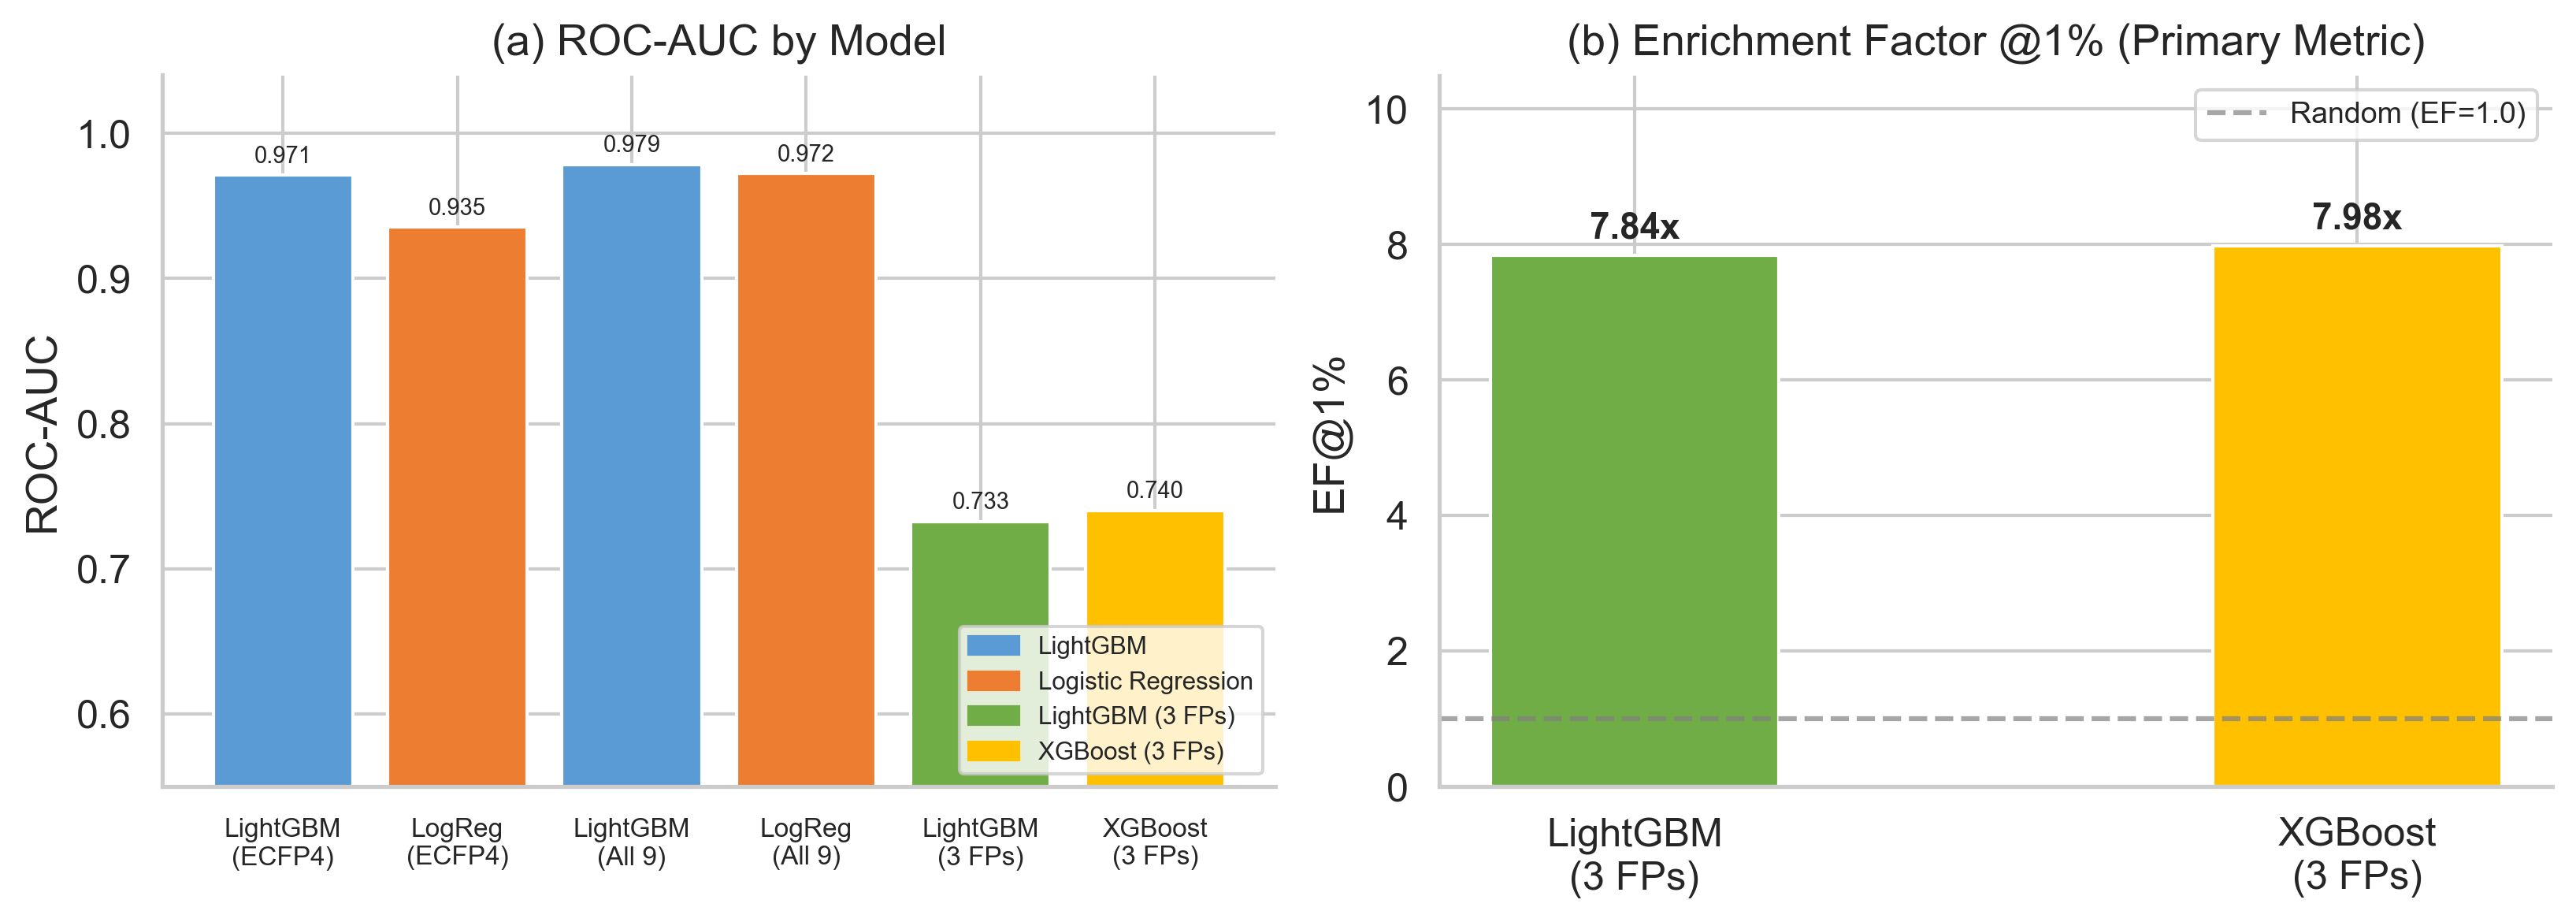
\includegraphics[width=\linewidth]{fig1_model_comparison.png}
\caption{Model comparison across feature sets and classifiers. (a) ROC-AUC for all six model configurations. (b) Enrichment Factor @1\% for models where it was measured; the dashed line indicates random baseline (EF = 1.0). XGBoost with ECFP6+MACCS+RDK achieves the highest EF@1\% of 7.98$\times$.}
\label{fig:model_comparison}
\end{figure}

\begin{table}[h]
\centering
\small
\caption{Test set performance of all models (stratified 80/20 split). EF@1\% is the primary challenge metric. Dashes indicate metrics not recorded for that experiment.}
\label{tab:results}
\begin{tabular}{llccccc}
\toprule
\textbf{Features} & \textbf{Model} & \textbf{ROC-AUC} & \textbf{PR-AUC} & \textbf{Bal.\ Acc.} & \textbf{Recall} & \textbf{EF@1\%} \\
\midrule
ECFP4 only      & LightGBM & 0.971 & 0.822 & 0.913 & 0.901 & -- \\
ECFP4 only      & LogReg   & 0.935 & 0.658 & 0.724 & 0.462 & -- \\
All 9 FPs       & LightGBM & 0.979 & 0.863 & 0.927 & 0.912 & -- \\
All 9 FPs       & LogReg   & 0.972 & 0.829 & 0.850 & 0.716 & -- \\
ECFP6+MACCS+RDK & LightGBM & 0.733 & 0.244 & 0.663 & 0.654 & 7.84 \\
ECFP6+MACCS+RDK & XGBoost  & 0.740 & 0.257 & 0.670 & 0.647 & \textbf{7.98} \\
\bottomrule
\end{tabular}
\end{table}

\subsection{Tanimoto Similarity and Ensemble}
The Tanimoto similarity scores against 177 known WDR91 actives are nearly uncorrelated with XGBoost scores (Pearson $r = -0.097$, Figure~\ref{fig:correlations}a), confirming that the two signals capture independent information: XGBoost learned from DEL binding patterns, while Tanimoto reflects drug-like scaffold similarity to confirmed binders. The ensemble of the two scores (rank-normalised, 60/40 weight) ranked all 339,258 Step~2 compounds; the top 1\% showed markedly elevated mean XGBoost (0.043 vs.\ 0.017 overall) and Tanimoto (0.292 vs.\ 0.199 overall) scores, indicating that top-ranked compounds are enriched for both DEL-like binding patterns and known-active scaffolds.

\begin{figure}[H]
\centering
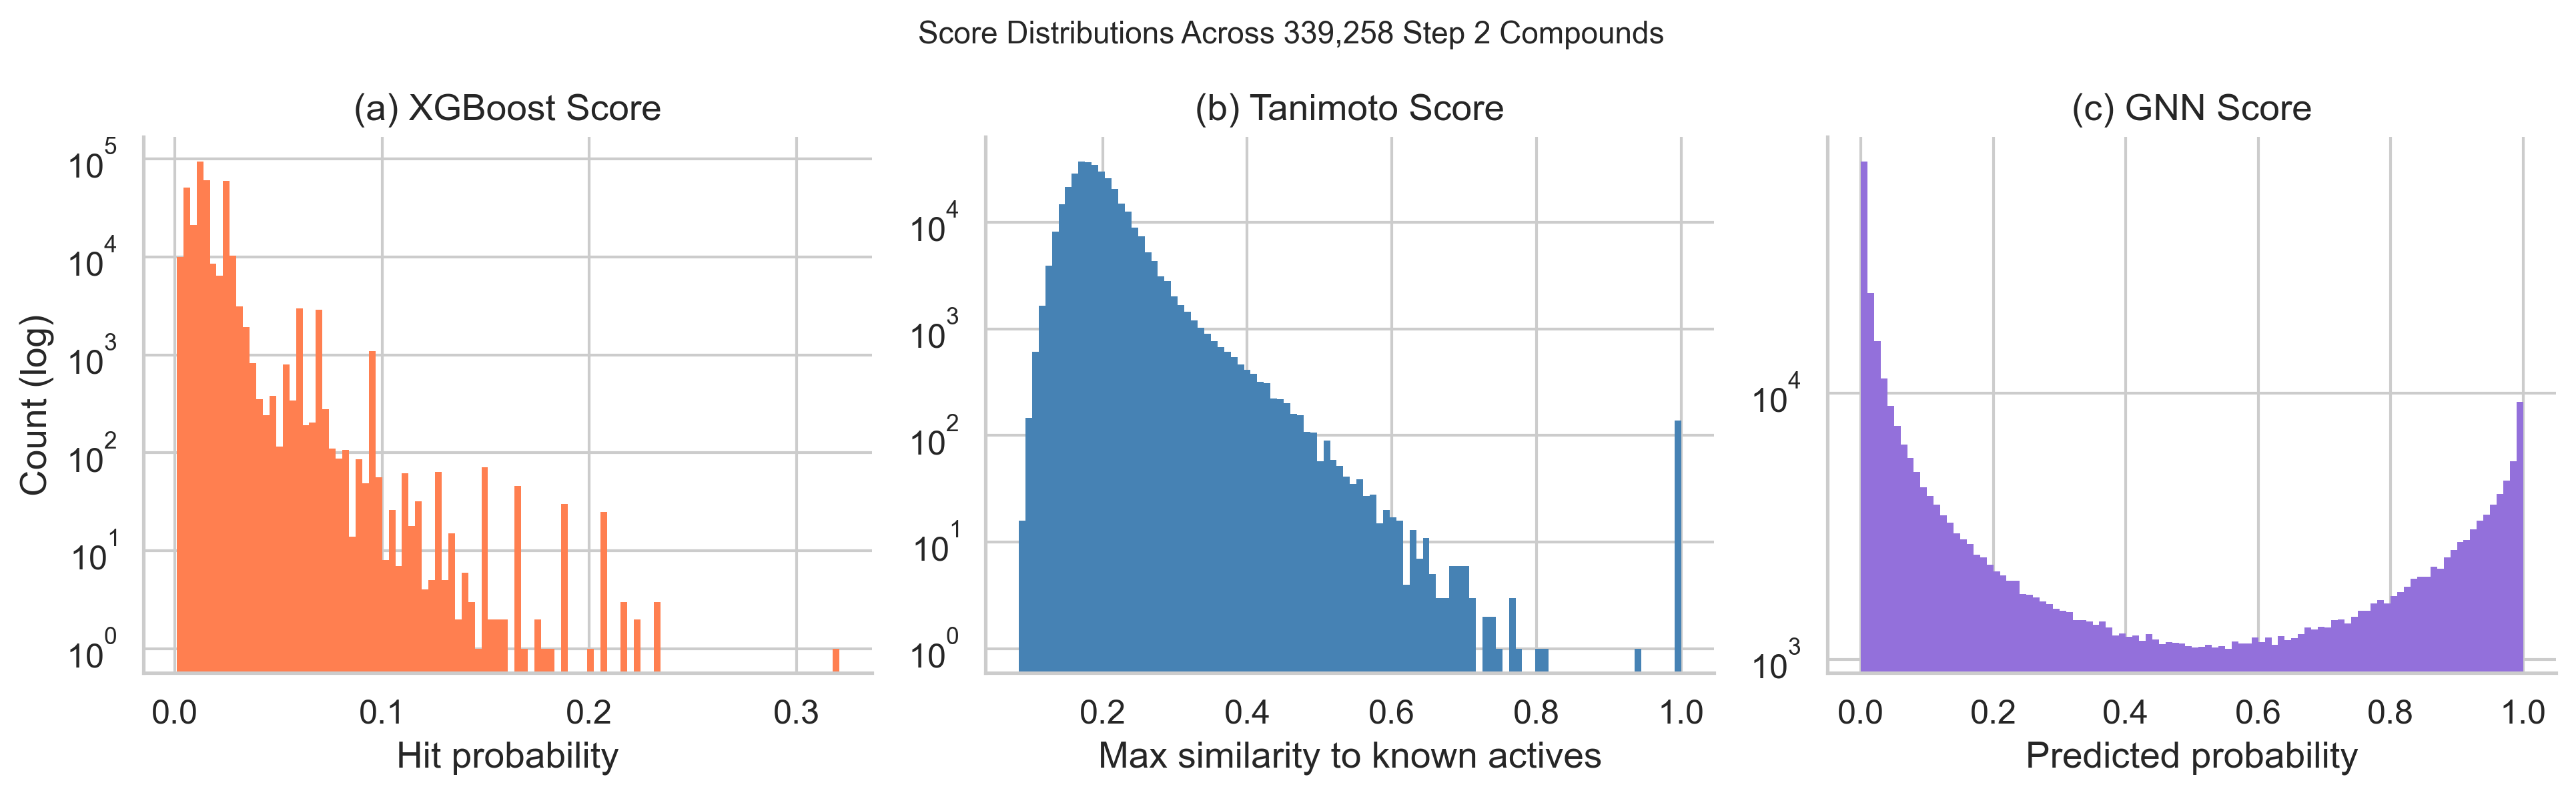
\includegraphics[width=\linewidth]{fig2_score_distributions.png}
\caption{Score distributions across all 339,258 Step~2 compounds (log-scale y-axis). (a) XGBoost hit probabilities are tightly clustered near zero due to class imbalance in the training data. (b) Tanimoto similarities to the 177 known actives are broadly distributed. (c) GNN pseudo-label probabilities are bimodal, reflecting the model's high confidence after training on pseudo-labelled SMILES.}
\label{fig:score_distributions}
\end{figure}

\subsection{GNN Pseudo-Labelling}
The GCN trained on pseudo-labelled Step~2 SMILES converged stably over 30 epochs. The GNN scores are moderately correlated with XGBoost scores (Pearson $r = 0.647$, Figure~\ref{fig:correlations}b), as expected since pseudo-labels are derived from XGBoost. Critically, the GNN top~1\% overlaps only 31.8\% with the XGBoost top~1\% and only 9.4\% with the XGBoost--Tanimoto ensemble top~1\% (Table~\ref{tab:overlap}, Figure~\ref{fig:overlap_importance}a). Of the 3,392 top-1\% GNN compounds, 2,000 appear in no other method's top list, while only 130 are shared by all three methods. This near-orthogonality suggests the GNN learned structural features from molecular graphs that are not captured by fixed-length fingerprints or Tanimoto similarity — consistent with prior work showing GNNs can identify binding motifs invisible to fingerprint-based methods~\cite{Gilmer2017}.

\begin{figure}[H]
\centering
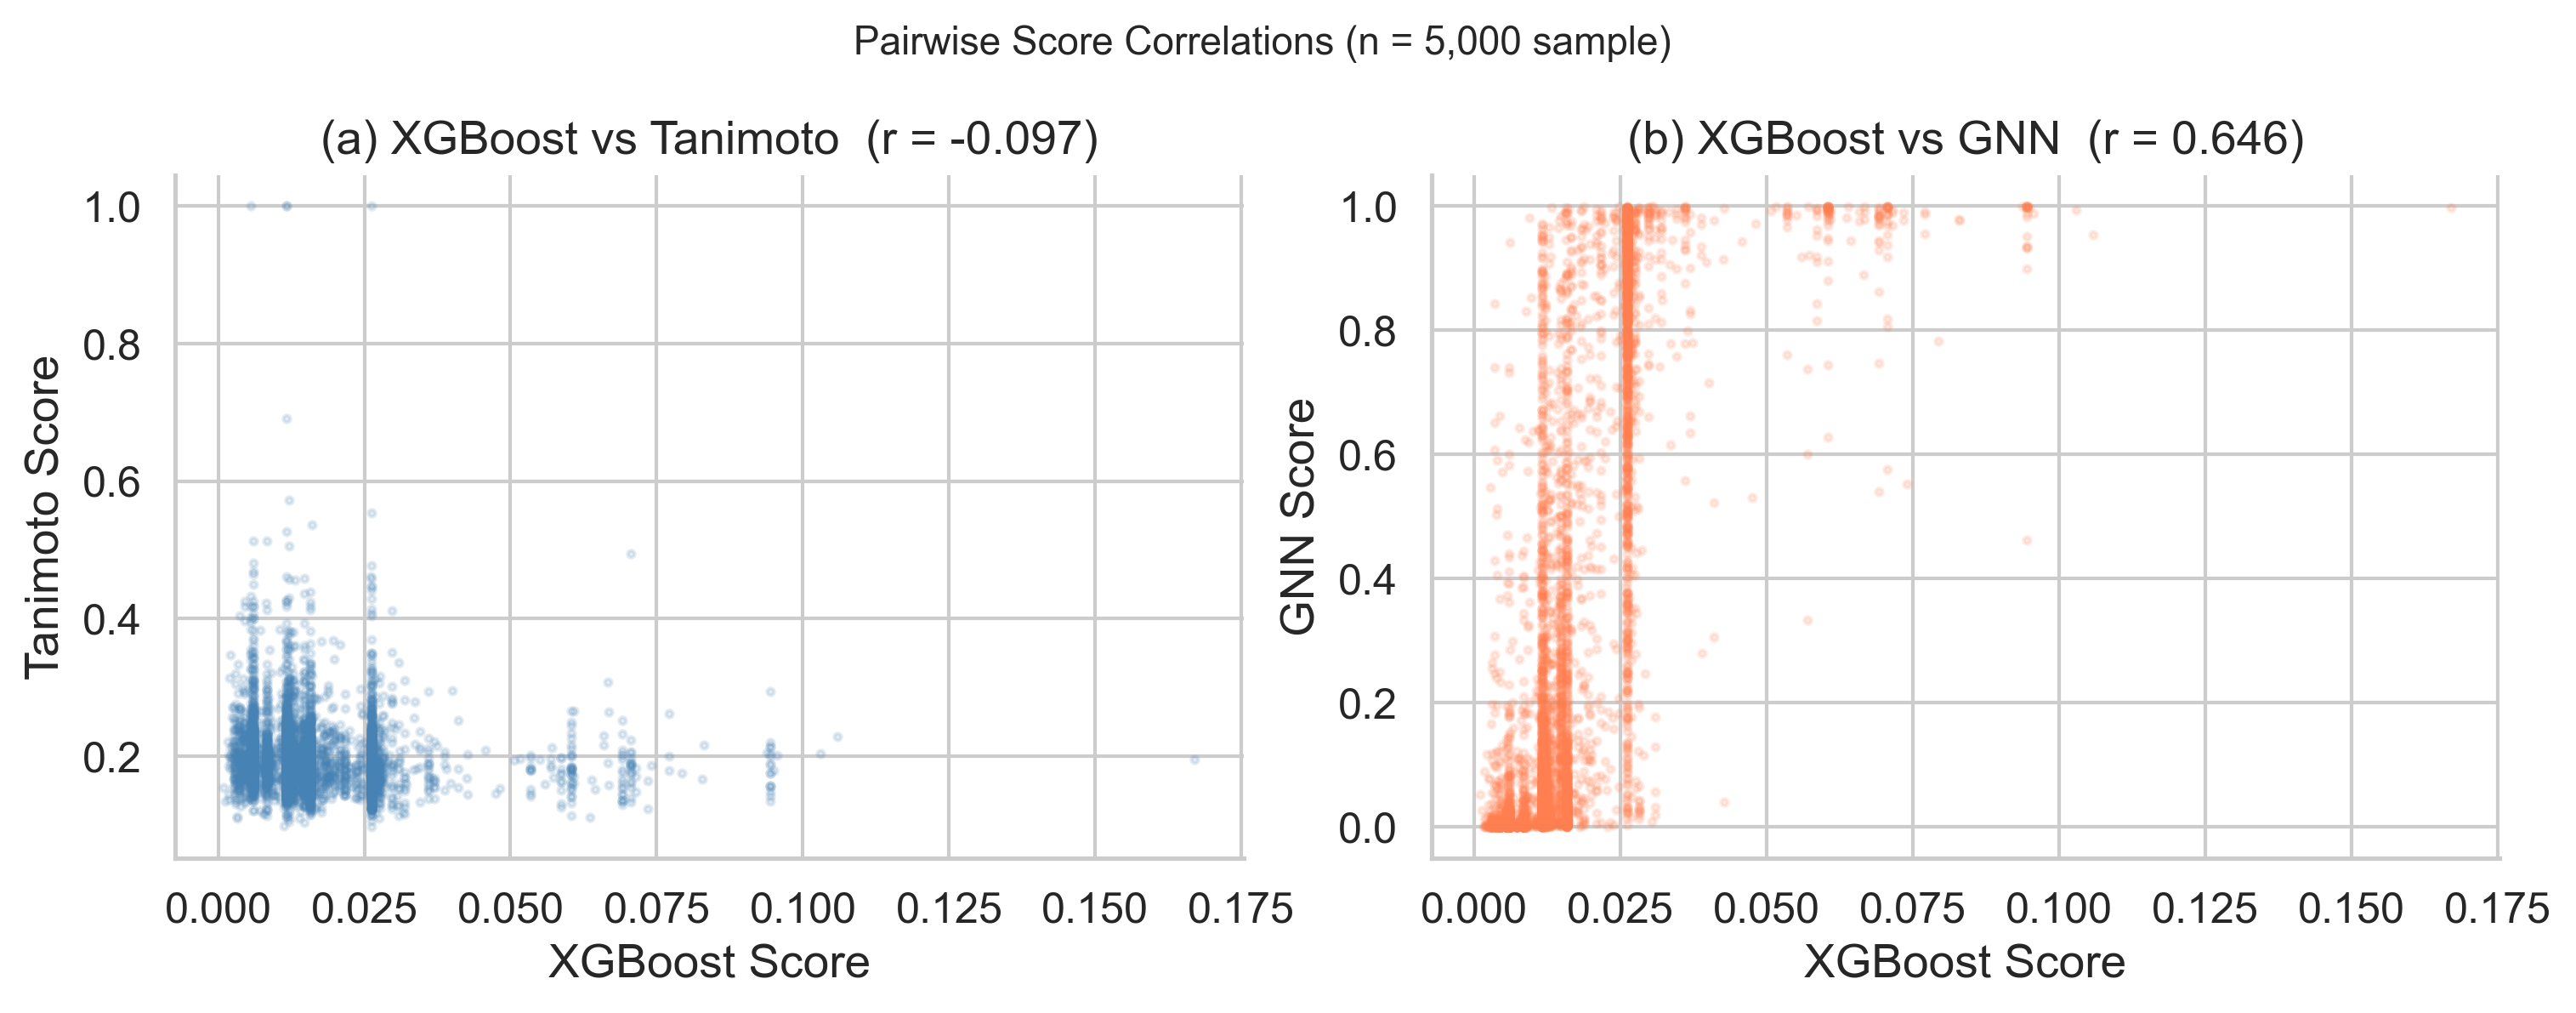
\includegraphics[width=\linewidth]{fig3_score_correlations.png}
\caption{Pairwise score correlations (n = 5,000 random sample). (a) XGBoost vs.\ Tanimoto scores show near-zero correlation ($r = -0.097$), confirming they capture independent signals. (b) XGBoost vs.\ GNN scores show moderate correlation ($r = 0.647$), expected since GNN pseudo-labels were derived from XGBoost predictions.}
\label{fig:correlations}
\end{figure}

\begin{figure}[H]
\centering
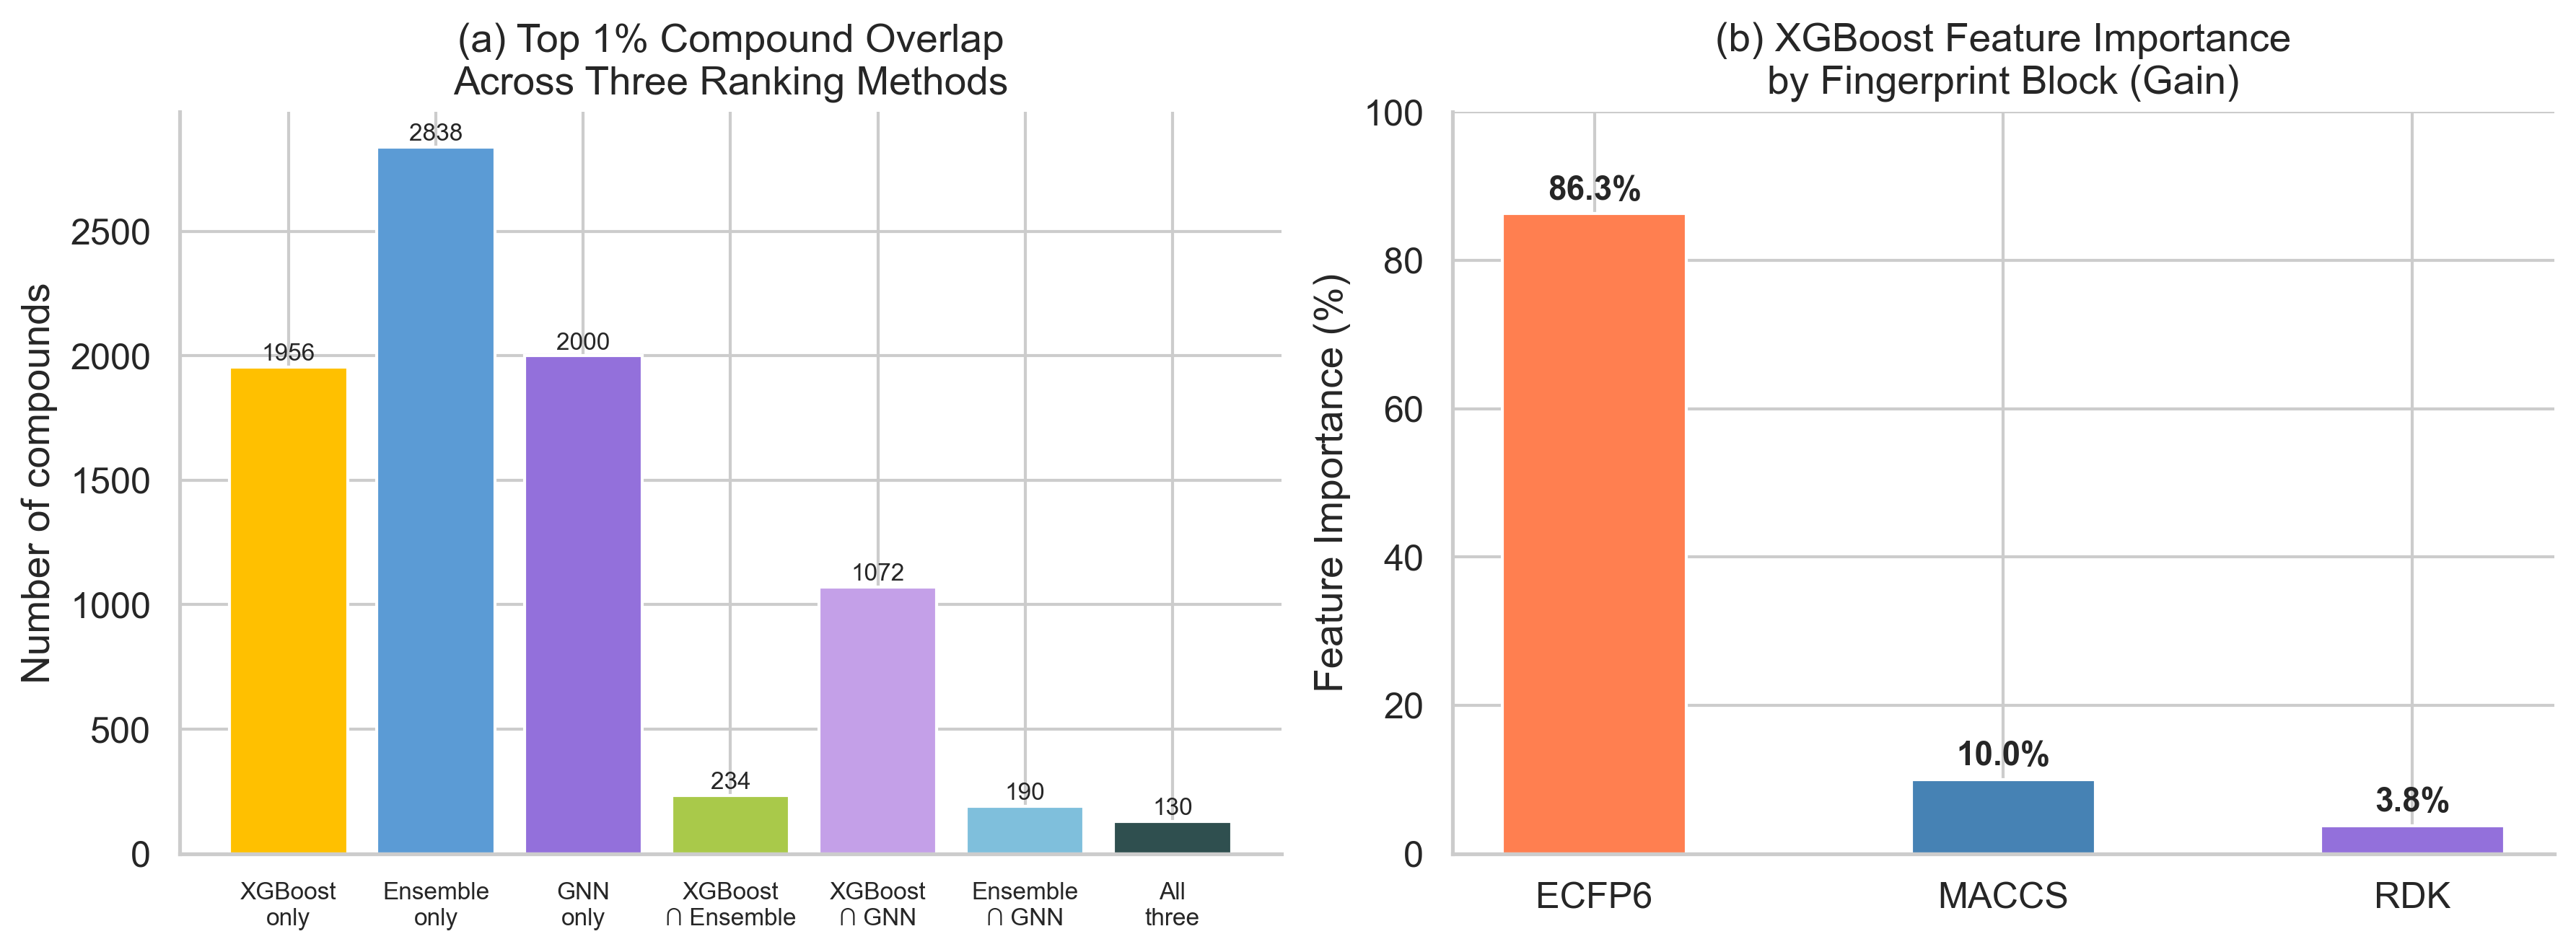
\includegraphics[width=\linewidth]{fig4_overlap_importance.png}
\caption{(a) Distribution of the top 1\% (3,392 compounds) across ranking methods. The majority of top candidates are method-specific, with only 130 compounds shared by all three methods, demonstrating complementary coverage of chemical space. (b) XGBoost feature importance by fingerprint block: ECFP6 dominates at 86.3\%, confirming circular fingerprints as the primary signal for WDR91 binding in DEL chemistry.}
\label{fig:overlap_importance}
\end{figure}

\begin{table}[h]
\centering
\small
\caption{Top 1\% overlap between ranking methods (339,258 Step~2 compounds; top 1\% = 3,392 compounds).}
\label{tab:overlap}
\begin{tabular}{lc}
\toprule
\textbf{Comparison} & \textbf{Overlap (\%)} \\
\midrule
GNN vs.\ XGBoost & 31.8 \\
GNN vs.\ XGBoost--Tanimoto Ensemble & 9.4 \\
XGBoost vs.\ XGBoost--Tanimoto Ensemble & -- \\
\bottomrule
\end{tabular}
\end{table}

% ── Discussion ────────────────────────────────────────────────────────────────
\section{Discussion}
Our results support the hypothesis that combining fingerprint-based learning, structural similarity to known binders, and graph-based learning identifies a broader set of candidate WDR91 binders than any single method. The EF@1\% of 7.98 for XGBoost on the DEL test set demonstrates strong ranking quality within the DEL chemical space.

The most striking finding is the low overlap between the GNN and ensemble top predictions (9.4\%). This suggests three distinct binding hypotheses are represented across the three methods: DEL-pattern-based (XGBoost), known-scaffold-based (Tanimoto), and graph-topology-based (GNN). Pooling these lists would diversify the experimental follow-up candidates and increase the probability of finding genuine WDR91 binders across different chemotypes.

The discrepancy between ROC-AUC and EF@1\% for XGBoost vs.\ LightGBM warrants discussion. The all-9-fingerprint LightGBM achieves ROC-AUC of 0.979 but was evaluated under a different experimental setup, preventing direct EF@1\% comparison. On a controlled identical split, LightGBM (ECFP6+MACCS+RDK) scores EF@1\% = 7.84 vs.\ XGBoost's 7.98. The difference is modest, but \texttt{scale\_pos\_weight} in XGBoost may provide a slight advantage by specifically upweighting the top of the ranking.

A key limitation is that the GNN pseudo-labels are noisy — they are derived from the same XGBoost model being compared. This introduces a feedback loop: compounds that XGBoost scores highly are more likely to receive pseudo-positive labels, so the GNN partly learns to replicate XGBoost's ranking. The 9.4\% overlap with the Tanimoto ensemble (which is independent of XGBoost for the structural similarity component) suggests the GNN does learn additional signal, but the extent cannot be quantified without ground-truth labels on Step~2.

A second limitation is the domain shift between training (DEL) and test (commercial library) chemistry. DEL compounds are combinatorial 3-building-block molecules, typically smaller and more polar than drug-like compounds. Our ECFP6 feature importance analysis (86.3\% of gain) confirms the model relies heavily on circular fingerprints that may not transfer well to novel scaffolds. The Tanimoto and GNN components were designed specifically to address this shift by incorporating drug-like chemical information.

Future work could include: (1) fine-tuning a pre-trained molecular transformer (e.g., ChemBERTa~\cite{Chithrananda2020}) on the 177 known actives as an additional ranking signal; (2) three-way score ensembling (XGBoost + Tanimoto + GNN); and (3) experimental validation of the top predictions through the SGC follow-up screen, which will provide ground-truth EF@1\% on the Step~2 library.

% ── References ────────────────────────────────────────────────────────────────
\bibliographystyle{unsrtnat}
\begin{thebibliography}{99}

\bibitem{Goodnow2017}
Goodnow, R.A., Dumelin, C.E., Keefe, A.D. (2017).
DNA-encoded chemistry: enabling the deeper sampling of chemical space.
\textit{Nature Reviews Drug Discovery}, 16(2), 131--147.

\bibitem{McCloskey2020}
McCloskey, K., Sigel, E.A., Kearnes, S., et al. (2020).
Machine learning on DNA-encoded library count data using an uncertainty-aware probabilistic loss function.
\textit{Journal of Chemical Information and Modeling}, 60(9), 4120--4130.

\bibitem{Jia2016}
Jia, D., Zhang, J., Li, F., et al. (2016).
Structural and mechanistic insights into regulation of the retromer coat by TBC1d5.
\textit{Nature Communications}, 7, 13305.

\bibitem{DREAM2035}
DREAM Target 2035 Drug Discovery Challenge. (2025).
\url{https://dreamchallenges.org/target-35-drug-discovery-challenge/}

\bibitem{Rogers2010}
Rogers, D., Hahn, M. (2010).
Extended-Connectivity Fingerprints.
\textit{Journal of Chemical Information and Modeling}, 50(5), 742--754.

\bibitem{Chen2016}
Chen, T., Guestrin, C. (2016).
XGBoost: A Scalable Tree Boosting System.
\textit{Proceedings of KDD 2016}, 785--794.

\bibitem{Ke2017}
Ke, G., Meng, Q., Finley, T., et al. (2017).
LightGBM: A Highly Efficient Gradient Boosting Decision Tree.
\textit{Advances in Neural Information Processing Systems}, 30.

\bibitem{Tanimoto1958}
Tanimoto, T.T. (1958).
An Elementary Mathematical Theory of Classification and Prediction.
IBM Internal Report.

\bibitem{RDKit}
Landrum, G. (2023).
RDKit: Open-source cheminformatics. \url{https://www.rdkit.org}

\bibitem{Gilmer2017}
Gilmer, J., Schütt, K.T., Brockherde, F., et al. (2017).
Neural Message Passing for Quantum Chemistry.
\textit{Proceedings of ICML 2017}, 1263--1272.

\bibitem{Fey2019}
Fey, M., Lenssen, J.E. (2019).
Fast Graph Representation Learning with PyTorch Geometric.
\textit{ICLR 2019 Workshop on Representation Learning on Graphs and Manifolds}.

\bibitem{Kipf2017}
Kipf, T.N., Welling, M. (2017).
Semi-Supervised Classification with Graph Convolutional Networks.
\textit{International Conference on Learning Representations (ICLR)}.

\bibitem{Chithrananda2020}
Chithrananda, S., Grand, G., Ramsundar, B. (2020).
ChemBERTa: Large-Scale Self-Supervised Pretraining for Molecular Property Prediction.
\textit{arXiv:2010.09885}.

\end{thebibliography}

\end{document}
